\documentclass[9pt]{report}

\usepackage{talks}
\newcommand{\expect}[1]{\mathbb{E}\!\left[ #1 \right]}
\newcommand{\reals}{\mathbb{R}}
\newcommand{\draw}[2]{#1^{(#2)}}
\usepackage{mathpazo}
\usepackage{sourcecodepro}

\begin{document}


\sf%
\mbox{ }
\\[12pt]
\spc{{\LARGE\bfseries \color{MidnightBlue}{Orders of Magnitude:}}}
\\[8pt]
\spc{\Large\bfseries \color{MidnightBlue}{Stan Algorithms and Engineering}}
\\[36pt]
\noindent 
\spc{\large\bfseries \color{MidnightBlue}{Bob Carpenter}}
\\[2pt]
\spc{\small Center for Computational Mathematics}
\\[2pt]
\spc{\small Flatiron Institute}
\vfill 
\noindent 
\spc{\footnotesize June 2023}
\hfill

\includegraphics[width=1.5in]{img/flatiron_logo.png}

\includegraphics[width=0.5in]{img/stan-logo.png}

\sld{Pop Quiz}
\begin{itemize}
\item Who's the most famous Stan in St.\ Louis?
\end{itemize}

\sld{Stan the Man \hfill (active 1941--1963 - WWII)}
\begin{itemize}
\item Not Ulam. Not a stalker fan.
\item \myemph{Stan ``The Man'' Musial}.  Outfielder, \myemph{\slshape St. Louis Cardinals.}
\end{itemize}
\begin{center}
  \spc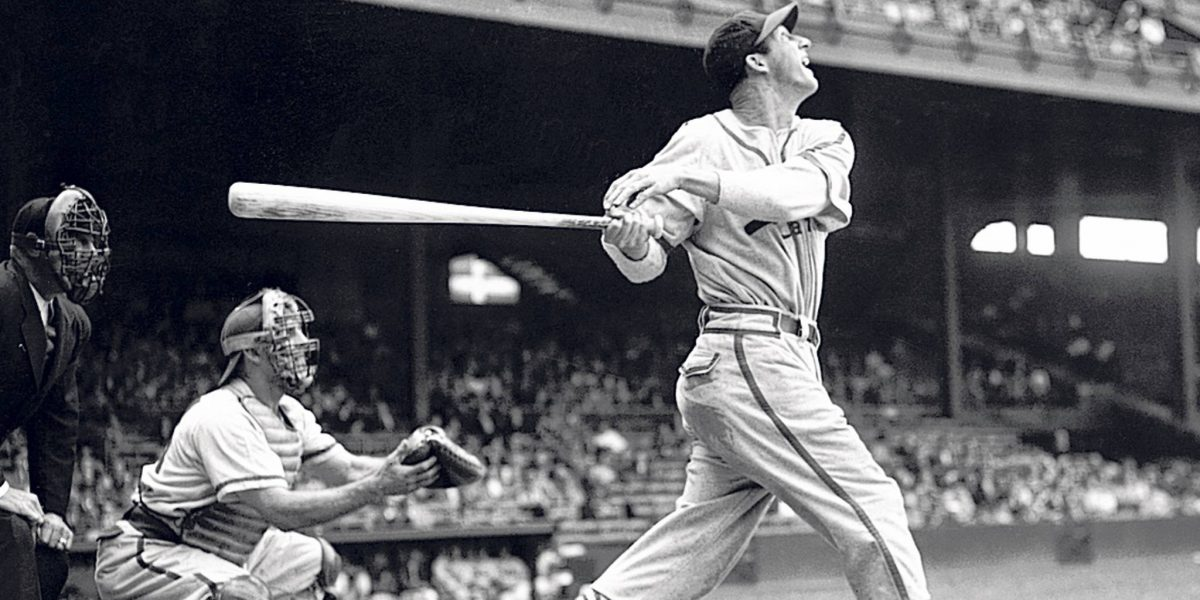
\includegraphics[width=0.6\textwidth]{img/stan-the-man.jpeg}
  \\
  {\small {\slshape Wikipedia}: One of the \myemph{greatest and most consistent} hitters in baseball}
  \end{center}


  \sld{}
  \vspace*{-24pt}
\begin{center}
    \spc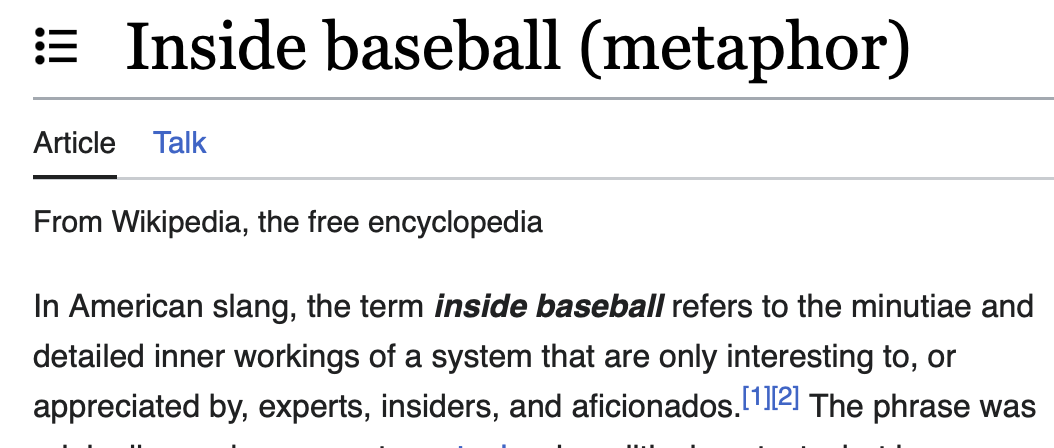
\includegraphics[width=\textwidth]{img/inside-baseball.png}
  \end{center}
  \vfill
  \null

  
\sld{Swing for the fences}
\begin{itemize}
\item 2011: I move \myemph{from industry to Columbia} to work with 
  Gelman. 
\item I was \myemph{getting scooped} on crowdsourcing. 
\item Michael Collins (CS) suggests I \myemph{work on harder problems}.
\item I \myemph{listened} and started the \myemph{Stan} project.
\end{itemize}
\begin{center}
  \spc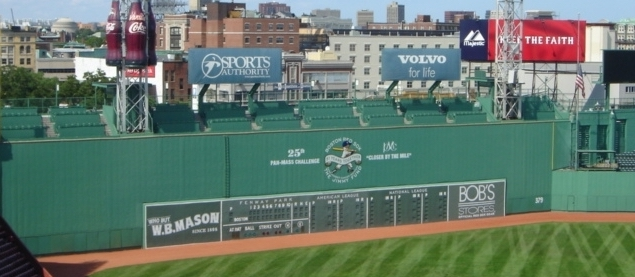
\includegraphics[width=0.6\textwidth]{img/fenway-fences.jpeg}
\end{center}


  
\sld{Where are the fences?}
\begin{itemize}
  \item \myemph{Sometimes}: an \myemph{unknown unknown}.
  \item \myemph{Usually}: about an \myemph{order of magnitude} away
  \item I'm a \myemph{computer scientist}, so that's only \myemph{$
      \mathbf{\times\, 2}$}  \hfill   ($\approx$\ Gelman \& Hill) 
  \end{itemize}
\vfill
\begin{center}
  \spc
  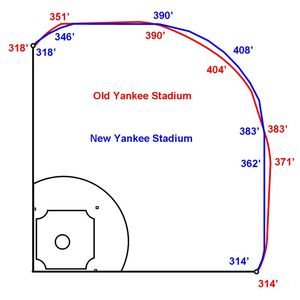
\includegraphics[height=1in]{img/yankee-stadium.jpeg}
  \hfill
  \spc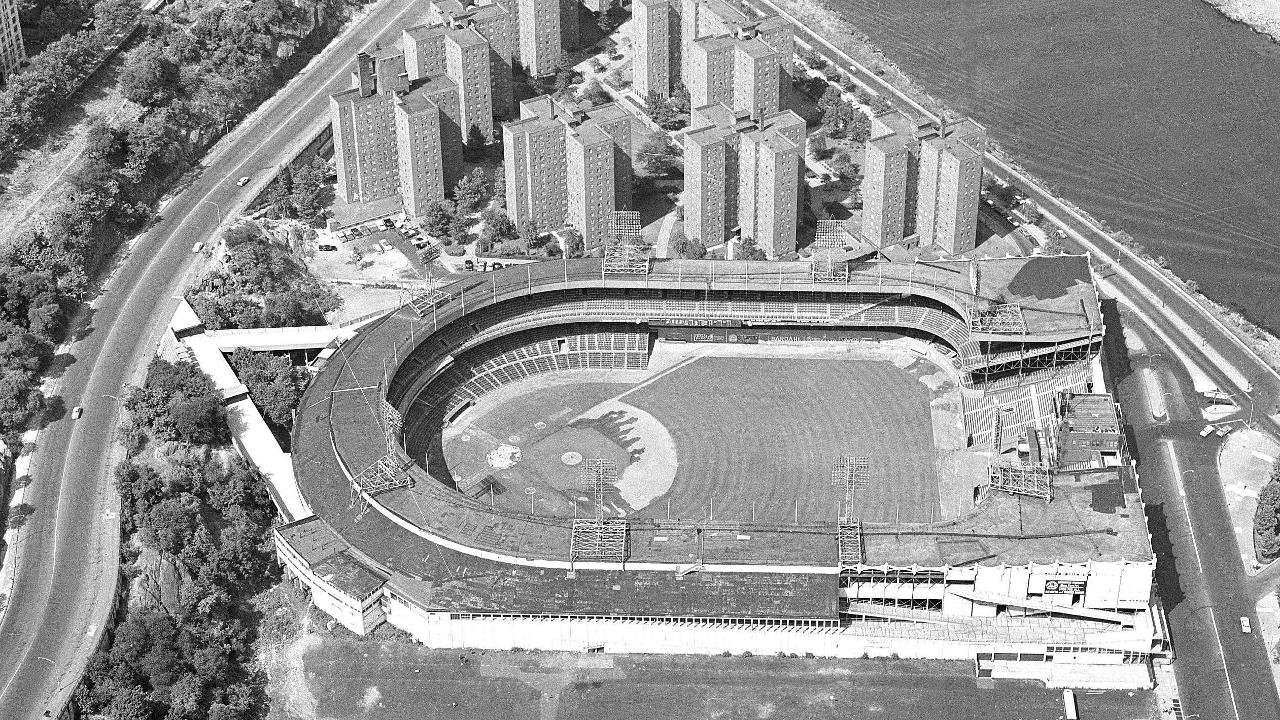
\includegraphics[height=1in]{img/polo-grounds.jpeg}
  \hfill
  \spc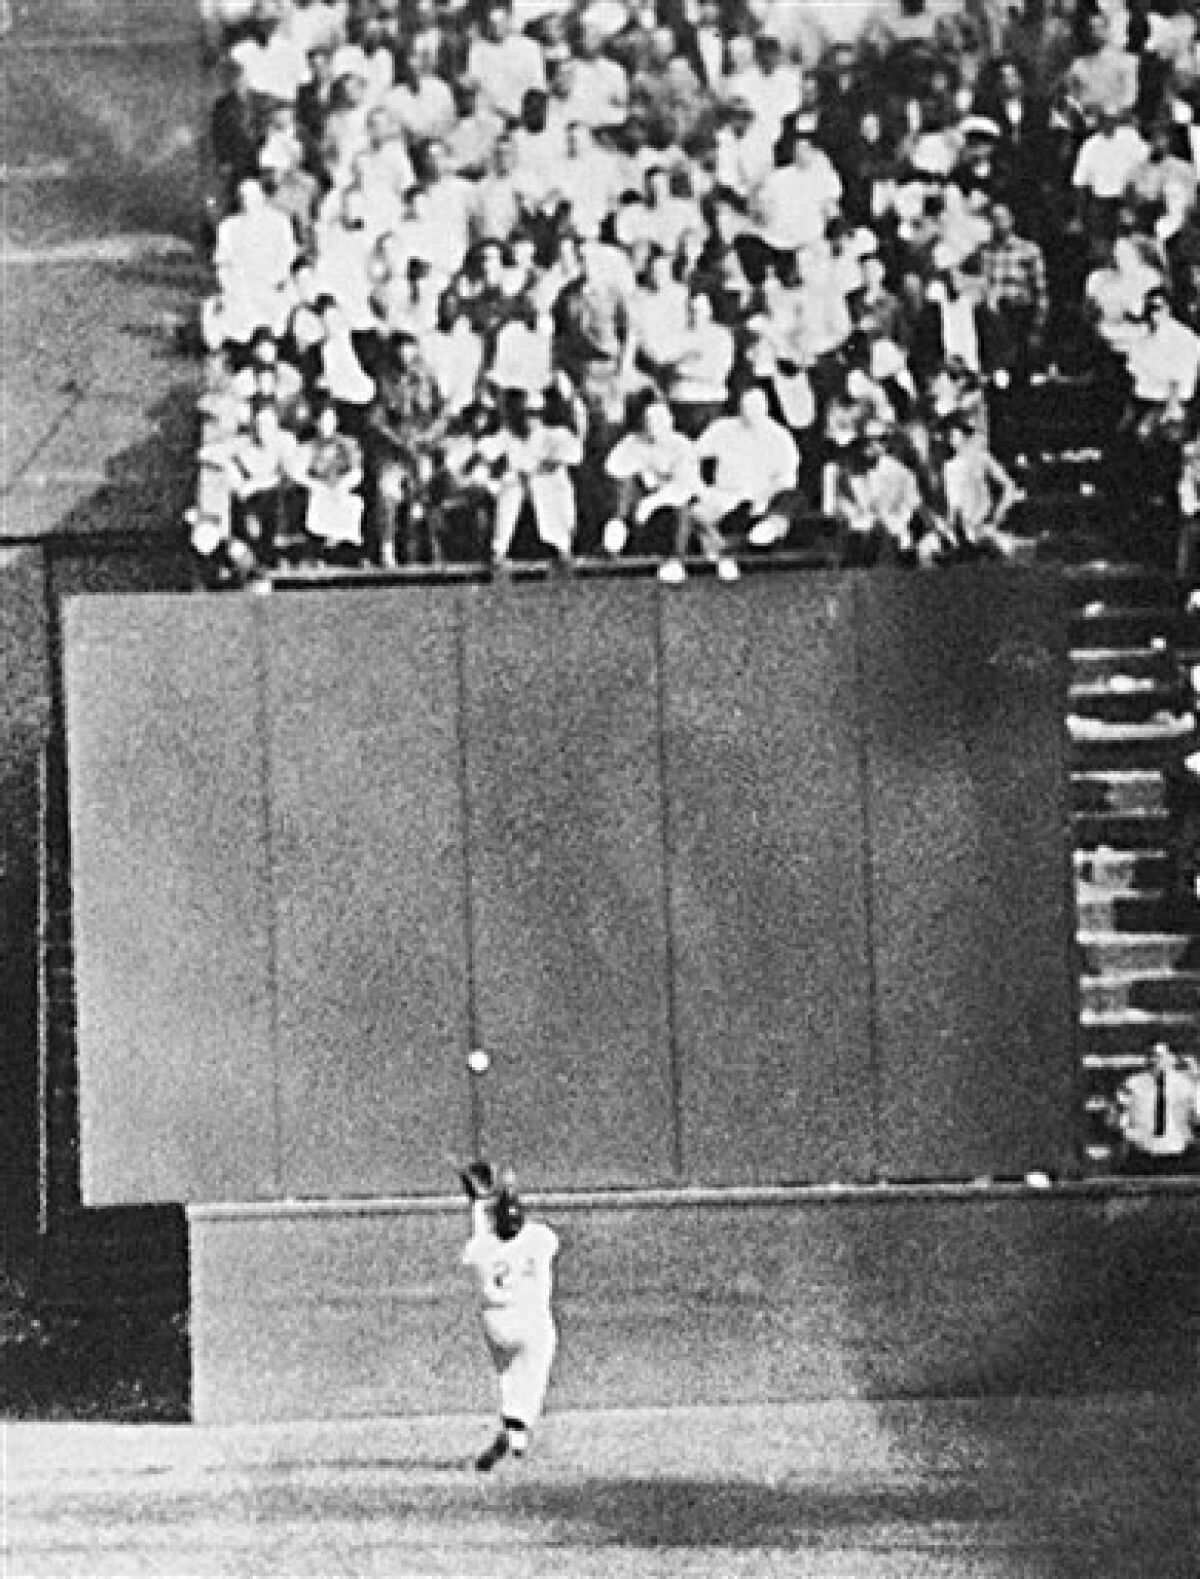
\includegraphics[height=1in]{img/willie-mays.jpeg}
\end{center}

\sld{}
\vfill
\begin{center}
\Huge \myemph{Part I\\[12pt] MCMC for Bayes}
\end{center}
\vfill
\vfill

\sld{Bayesian Inference \hfill\normalsize (Bayes $\approx$ 1750,
  Laplace $\approx$ 1800)}
\begin{itemize}
\item unknown (parameters) $\theta \in \reals^D;$ \quad 
  observed (data) $y \in \reals{N}$
\item \myemph{Estimation}: 
$$
\widehat{\theta}
= \expect{\theta \mid y}
= \int_{\reals^D} \theta \cdot p(\theta \mid y) \textrm{d}\theta. 
$$
\item \myemph{Event probabilities}
$$
\Pr[A \mid y]
= \expect{\textrm{I}_{A}(\theta) \mid y}
= \int_{\reals^D} \textrm{I}_{A}(\theta) \cdot p(\theta \mid y) \, \textrm{d}\theta. 
$$
\item \myemph{Posterior prediction}
$$
p(\tilde{y} \mid y) 
= \expect{p(\tilde y \mid \theta) \mid y}
= \int_{\mathbb{R}^D} p(\tilde{y} \mid \theta) \cdot p(\theta \mid 
  y) \, \textrm{d}\theta. 
$$
\end{itemize}

\sld{Monte Carlo \hfill {\normalsize (Fermi, von Neumann, Ulam
    $\approx$ 1930s--1940s)}}
\begin{itemize}
\item Go-to approach to \myemph{high-dimensional integration}
\item \myemph{Randomized algorithm} for deterministic integrals 
$$
\expect{f(\theta)] \mid y}
\approx \frac{1}{M} \sum_{m = 1}^M f\!\left(\draw{\theta}{m}\right) 
$$
for 
$$
\draw{\theta}{m} \sim p(\theta \mid y) 
$$
\myemph{independent and identically distributed} (i.i.d.) 
\item Proof: \myemph{central limit theorem}
  + law of \myemph{unconscious statistician}. 
\end{itemize}

\sld{Markov chain Monte Carlo \hfill \normalsize(Ulam, late 1940s)}
\begin{itemize}
\item When \myemph{too hard to draw i.i.d.}\ from posterior.
\item Draw $\draw{\theta}{0}, \ldots, \draw{\theta}{M}$ from a
  homogeneous \myemph{Markov chain}
\begin{align}
\draw{\theta}{0} &\sim q_0(\theta)
  \\[8pt]
  \theta_{m + 1} &\sim q(\theta_{m + 1} \mid \theta_{m}).
\end{align}
\item Evaluate with averages like Monte Carlo, when Markov chain 
  \begin{subitemize}
  \item is \myemph{irreducible} (doesn't get stuck),
  \item is \myemph{aperiodic} (doesn't visit partition cyclically), and
  \item has \myemph{stationary distribution} s.t.\
    $\draw{\theta}{m + 1} \sim p(\theta \mid y)$ if
    $\draw{\theta}{m} \sim p(\theta \mid y).$
  \end{subitemize}
\item Proof: MCMC CLT + law of unconscious statistician
\end{itemize}

\sld{Accept/reject balance \hfill \normalsize(Metropolis et al.\ 1950)}
\begin{itemize}
\item \myemph{propose} $\theta^* \sim q(\theta \mid \theta_{m})$,  
  \begin{subitemize}
  \item where $q$ is \myemph{symmetric}, i.e.,  $q(\theta' \mid \theta) = q(\theta \mid \theta')$
  \end{subitemize}
  \item \myemph{accept} with probability  
$\displaystyle  
\min\!\left( 1,  \
  \frac{p(\theta^* \mid y)}
       {p(\theta_m \mid y)}
     \right)$
\renewcommand{\baselinestretch}{1.2}
{\small\bfseries
\begin{verbatim} 
theta[0] = q0_rng()
for m in range(M):
   theta_star = q_rng(theta[m])
   u = uniform_rng(0, 1)
   accept = log(u) < log p(theta_star) - log p(theta[m])
   theta[m + 1] = theta_star if accept else theta[m]
\end{verbatim}
}
\renewcommand{\baselinestretch}{1.0}
\end{itemize}

\sld{Non-reversible proposals \hfill \normalsize (Hastings 1970)}
\begin{itemize}
\item \myemph{propose} $\theta^* \sim q(\theta \mid \theta_{m})$, 
  \begin{subitemize}
  \item where $q$ is \myemph{not necessarily symmetric}
  \end{subitemize}
  \item \myemph{accept} with probability 
$\displaystyle 
\min\!\left( 1, 
  \frac{p(\theta^* \mid y)}{p(\theta_m \mid y)}
    \cdot 
    \frac{p(\theta_m \mid \theta^*)}{p(\theta^* \mid \theta_m)}
     \right)t$
\item If $q$ is symmetric, second term drops out, left with Metropolis
\end{itemize}

\sld{Detailed Balance}
\begin{itemize}
\item Let $p(\theta_{m + 1} \mid \theta_m)$ be the Markov chain
  \myemph{transition kernel}
  \begin{subitemize}
  \item reject probability makes it mixed discrete/continuous
  \end{subitemize}
\item MH accept ensures MCMC kernel satisfies
  \myemph{detailed balance},
  $$
  p(\theta \mid y) \cdot p(\theta' \mid \theta)
  = p(\theta' \mid y) \cdot p(\theta \mid \theta').
  $$
  \vspace*{-12pt}
  \begin{subitemize}
    \item ensures chain has stationary distribution $p(\theta \mid y)$
    \item given irreducibility and aperiodicity
      \end{subitemize}
\end{itemize}

\sld{HMC \hfill \normalsize(Duane et al.\ 1987)}
\begin{itemize}
\item \myemph{couples momentum} $\rho \in \mathbb{R}^D$ to sample over
  \myemph{phase space} $\reals^D \times \reals^D$
\item \myemph{Hamiltonian} $H(\theta, \rho) = - \log p(\theta, \rho) =
  - \log p(\theta) - \log p(\rho),$
  \begin{subitemize}
  \item \myemph{Kinetic energy}: $-\log p(\rho) = -\log \textrm{normal}(0, \textrm{I}_D) =
    \frac{1}{2}
    \cdot \theta^{\top} \cdot \theta.$
  \item \myemph{Potential energy}: $-\log p(\theta) = - \log p(\theta \mid y)$
  \end{subitemize}
\item \myemph{Hamiltonian Monte Carlo} (HMC) couples two stationary-preserving transition kernels:
  \begin{subitemize}
  \item \myemph{Exact momentum} refresh: $\rho_{m + 1} \sim \textrm{normal}(0, 1).$
  \item \myemph{Metropolis proposal}: $(\theta^*,
    -\rho^*)$, where $(\theta^*, \rho^*)$ solves Hamiltonian dynamics from initial
    $(\theta_m, \rho_{m + 1})$ to proposal $(\theta^*, \rho^*)$ at
    time $t$.
  \item Metropolis \myemph{corrects numerical integration error} solving ODE
  \item Momentum \myemph{flip for reversibility}
  \end{subitemize}
\end{itemize}

\sld{Why is HMC so good?}
\begin{itemize}
\item Its Metropolis steps makes large distance proposals with high
  acceptance rates
\item \myemph{Effective sample size} (and hence \myemph{mixing}) is proportional to expected squared
  jump distance
\item An \myemph{exact solution} preserves initial Hamiltonian, so 100\% accept 
\item The \myemph{leapfrog integrator} used to solve dynamics is \myemph{symplectic}
  \begin{subitemize}
    \item steps preserve volume (hence no Hastings correction for Jacobian)
    \item symplectic integrators very good at \myemph{preserving Hamiltonian}
    \item not so great at \myemph{solving dynamics}, but doesn't matter---we
      only need \myemph{big jumps with high acceptance}
  \end{subitemize}
\end{itemize}

\sld{HMC + Euclidean metric}
\begin{itemize}
\item add symmetric, positive-definite \myemph{metric} $M$ to
  define distance
  $$
  d(\theta, \theta') = (\theta - \theta')^{\top} \cdot M \cdot (\theta
  - \theta').
  $$
\item Stan estimates $M$ as inverse posterior covariance,
  $$
  \widehat{M} = \textrm{cov}[\theta \mid y].
  $$
\item \myemph{kinetic energy} now $-\log p(\rho) = \frac{1}{2} \cdot \rho^{\top} \cdot M \cdot \rho,$
\item so \myemph{momentum refresh} $\rho \sim \textrm{normal}(0, M^{-1}).$
\end{itemize}


\sld{No-U-Turn Sampler \hfill \normalsize (Hoffman and Gelman 2013)}
\begin{itemize}
\item \myemph{Tuning HMC} dynamics (step size, number of steps) is
  \myemph{very hard}
\item NUTS auto tunes
  \begin{subitemize}
  \item \myemph{stepsize} during warmup iterations
  \item \myemph{number of steps} dynamically
  \item \myemph{metric} during warmup iterations (revision)
  \end{subitemize}
\item Sampling algorithm
  \begin{subitemize}
  \item simulate \myemph{forward or backward} time at random, \myemph{double steps} each time
  \item \myemph{until U-turn} (ends' momentum brings them closer)
  \item \myemph{select a step} along path, \myemph{biased} toward \myemph{last
        doubling}
    \item \myemph{slice sampling}, revised to more efficient \myemph{multinomial}
    \end{subitemize}
\end{itemize}

\sld{Generalized HMC \hfill \normalsize (Horowitz 1991)}
\begin{itemize}
\item Uses \myemph{partial momentum refresh}
  \begin{subitemize}
    \item preserves momentum for directed movement across posterior
    \end{subitemize}
\item Fix $\lambda \in (0, 1)$ (lower preserves more momentum)
\item \myemph{G-HMC refresh}:
  $$
  \rho_{m + 1} = \sqrt{\lambda} \cdot z_m + \sqrt{1 - \lambda}
  \cdot \rho_m,
  $$
where $z_m \sim \textrm{normal}(0, \textrm{I}_D).$
\item This is also an \myemph{exact update}
  \begin{subitemize}
    \item i.e., if $\rho_m \sim  \textrm{normal}(0, \textrm{I}_d),$ then $\rho_{m + 1} \sim 
    \textrm{normal}(0, \textrm{I}_d).$
    \end{subitemize}
\end{itemize}

\sld{Uh oh!  What about the Flip?}
\begin{itemize}
\item \myemph{Why not} use G-HMC with a single step and tune $\lambda$?
\item Remember that \myemph{momentum flip}?
  \begin{subitemize}
  \item it's required for \myemph{reversibility} of Metropolis
  \item \myemph{thrown away} in basic HMC by composing momentum update
  \item but \myemph{preserved} in G-HMC
  \end{subitemize}
\item \myemph{Without high acceptance}, momentum flip produces \myemph{random walk}. 
\item High acceptance means \myemph{small steps} in Hamiltonian dynamics.
\end{itemize}

\sld{Non-reversible accept \hfill \normalsize(Neal 2020)}
\begin{itemize}
\item Instead of uniform $u$, use \myemph{sawtooth}, \myemph{perturbed} for ergodicity
  \begin{subitemize}
  \item \myemph{not reversible}, but \myemph{preserves stationary}
  \end{subitemize}
\item Iteration vs.\ $u$ (red reject) shows grouped acceptance:
\begin{center}
  \spc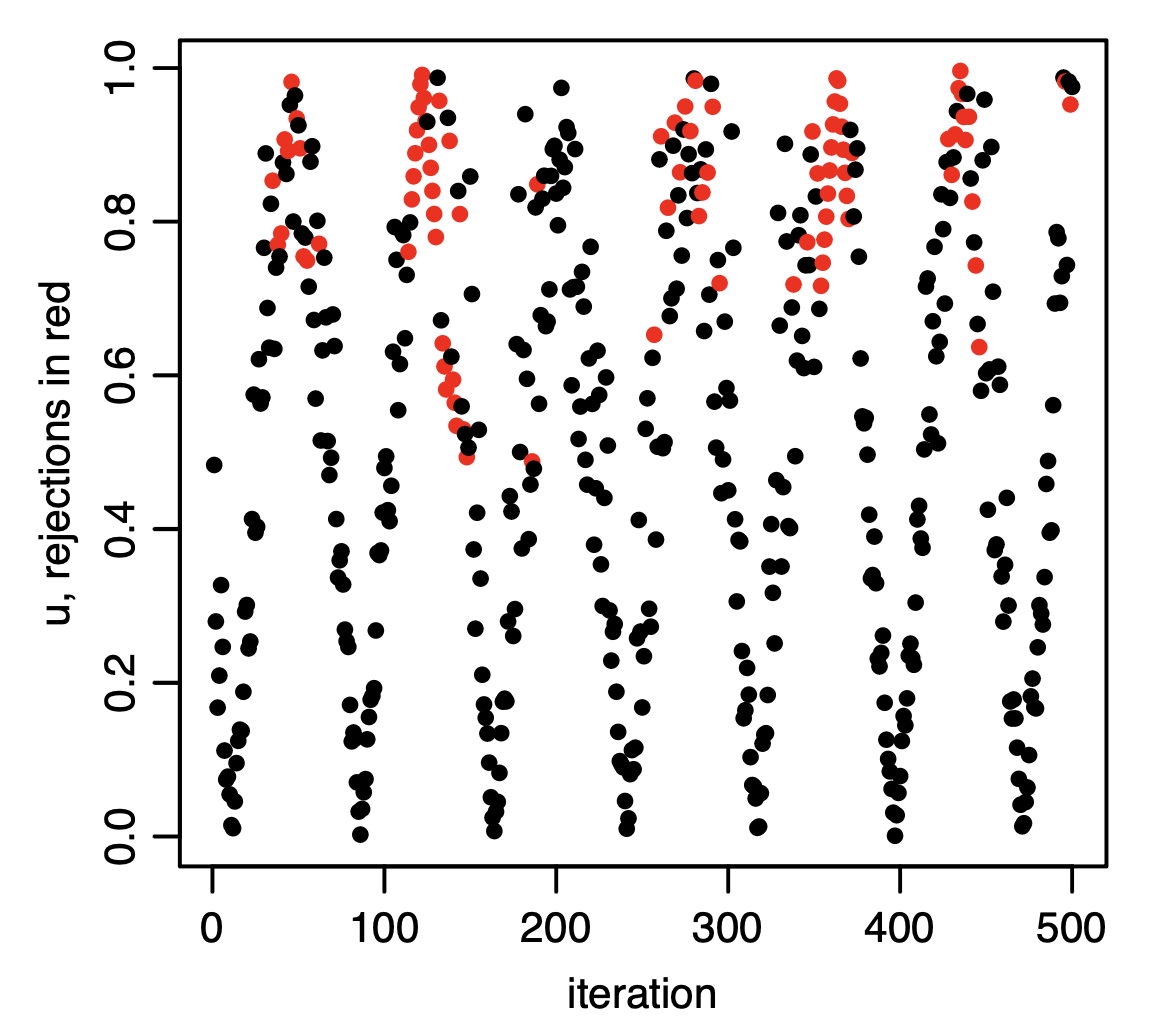
\includegraphics[height=1.5in]{img/neal-nonrevu.png}
\end{center}
\end{itemize}

\sld{Delayed Rejection \hfill \normalsize(Mira 2001)}
\begin{itemize}
\item $K$-step delayed rejection involves $K$ distinct proposals
  \begin{subitemize}
\item Step 1.  Propose and accept/reject as usual with Metropolis.
\item Step 2.  \myemph{If rejected, propose again} with a new proposal
  and accept/reject with \myemph{Metropolis-Hastings}
\item Step 3.  If rejected again, propose again.
\\
\qquad \qquad    $\vdots$
\item Step $K$.  If rejected, propose one last time.
\end{subitemize}
\item Need \myemph{Hastings correction} to ensure detailed balance.
\item Proposals may depend on previous proposal(s).
\end{itemize}

\sld{Delayed Rejection HMC \hfill \normalsize(Modi et al.\ 2022)}
\begin{itemize}
\item Just what it \myemph{says on the tin}: DR applied to HMC
\item Each \myemph{retry cuts step size} by constant $c$ and \myemph{multiplies steps}
  by $c$ (e.g., $c = 2$ or $c = 5$)
  \begin{subitemize}
  \item earlier attempts kept step size and extended path
  \item our approach better if rejection was because Hamiltonian
    diverged
  \item divergence is when step size isn't small enough for
    first-order gradient-based approximations to deal with curvature
  \end{subitemize}
\item \myemph{Chirag's DR innovation:} Only retry if acceptance probability for
  previous try was low.
\item Deals with *multiple scales* (varying curvature
  direction/magnitude) \myemph{along an entire path}.
\end{itemize}

\sld{MEADS \hfill \normalsize(Hoffman and Sountsov 2022)}
\begin{itemize}
\item \myemph{Massively parallel} version of Neal's non-reversible
  accept form of \myemph{G-HMC}
\item Uses \myemph{complementary chains for adaptation}
  \begin{subitemize}
  \item novel, efficient \myemph{principal eigenvalue} estimation of
    step size
  \item covariance in complementary chains used to \myemph{estimate metric}
  \item \myemph{accelerates adaptation}, robust to single chains getting stuck (Bales 2019)
  \end{subitemize}
\item conveniently a Markov chain \myemph{w.o.\ warmup phase}
\end{itemize}

\sld{DR-G-HMC \hfill \normalsize(Modi et al. in progress)}
\begin{itemize}
\item Apply delayed rejection to generalized HMC with one step.
\item Retries only use a single step.
\item Deals with multiple scales \myemph{within a path}
\item Use MEADS-like tuning.
\end{itemize}

\end{document}
